\documentclass{article}

% if you need to pass options to natbib, use, e.g.:
%     \PassOptionsToPackage{numbers, compress}{natbib}
% before loading neurips_2026

% Submission/track options (see neurips_2026.sty header).
% We use the "preprint" track so author identity is shown, line numbers
% are removed, and the footer reads "Preprint. Work in progress." which
% is appropriate for a graded course report rather than a blind review.
\usepackage[preprint]{neurips_2026}

\usepackage[utf8]{inputenc}
\usepackage[T1]{fontenc}
\usepackage{hyperref}
\usepackage{url}
\usepackage{booktabs}
\usepackage{amsfonts}
\usepackage{amsmath}
\usepackage{amssymb}
\usepackage{nicefrac}
\usepackage{microtype}
\usepackage{xcolor}
\usepackage{graphicx}
\usepackage{tikz}
\usetikzlibrary{positioning, arrows.meta, shapes.geometric, fit, backgrounds, calc}
\usepackage{multirow}
\usepackage{caption}
\usepackage{subcaption}
\usepackage{float}
\captionsetup{font=small, labelfont=bf}
\graphicspath{{figures/}}

\title{Re-Implementing CNN Price-Trend Signals:\\
A Reproduction of Jiang, Kelly, and Xiu (2023)}

\author{%
  Kaibiao Zhu \\
  Final Project, Machine Learning for Finance \\
  The Hong Kong University of Science and Technology (Guangzhou) \\
  \texttt{kzhu597@connect.hkust-gz.edu.cn}
}


\begin{document}


\maketitle


\begin{abstract}
This paper reproduces the image-based price-trend prediction framework of
\citet{jiang2023reimagining} (hereafter the \emph{original paper}), which replaces predefined technical indicators
with OHLC-volume charts and convolutional neural networks (CNNs). Using CRSP
daily U.S. equity data, we reconstruct the image pipeline, train horizon-specific
CNN ensembles, and evaluate the resulting signals through out-of-sample backtests. We compare the CNN signals with momentum,
moving-average, and reversal benchmarks, and assess residual performance through
factor-spanning regressions. The reproduction is strongest at short horizons,
where image-based signals deliver the best economic performance. Relative to
the magnitudes reported by the original paper, medium- and
long-horizon strategies weaken substantially after costs, and factor stripping
yields significantly negative alphas. Saliency
maps indicate that the CNN mainly attends to recent price movement and volume
contrast. We also provide replication materials so that the empirical results
can be audited and extended.
\end{abstract}


\section{Introduction}
\label{sec:intro}

Technical analysis has long suggested that the visual ``shape'' of a price
chart conveys information beyond what is captured by scalar momentum or
moving-average filters. The original paper formalises this intuition
by feeding fixed-resolution open--high--low--close (OHLC) images with a
volume sub-panel into a convolutional neural network and showing that the
resulting forecasts dominate canonical price-trend signals out of sample.
The study joins a growing empirical asset-pricing literature that uses
flexible machine-learning predictors to map raw historical features into
expected returns \citep{gu2020empirical,kelly2019characteristics}, and it
ties directly to early efforts at formalising chart patterns via kernel
smoothing \citep{lo2000foundations}.

This paper re-implements the core pipeline from end to end and evaluates it
under the same in-sample and out-of-sample calendar design as
the original paper: training and validation draw from 1993--2000
with a 70/30 random sample split, and headline out-of-sample results are
reported for 2001--2019. Our contributions are:
\begin{enumerate}
  \item An independent OHLC-plus-volume image renderer and horizon-matched CNN
        stacks built from the dimensions, drawing rules, and layer geometry
        documented in the original paper---including the simple
        moving-average overlay, volume sub-panel, and vertical orientation
        convention---implemented from the original paper's written specification and
        reported tensor dimensions.
  \item A CRSP-style daily panel for data construction, with headline
        out-of-sample CNN evaluation as above; proportional transaction
        costs; matched-horizon price momentum, simple moving-average cross,
        and short-term reversal baselines; and a five-factor-plus-momentum
        spanning regression \citep{fama1993common,fama2015five,carhart1997persistence}.
  \item Input-gradient saliency analysis \citep{simonyan2014deep} of the
        $I=60$ ensemble, which highlights the right tail of each image and
        the volume bars as the dominant feature regions.
  \item Code, trained weights, and post-aggregation CSV tables are released
        on \href{https://github.com/George-hardworking/machine-learning-for-finance/tree/main/final_submit_version}{GitHub},
        allowing every numerical claim to be regenerated.
\end{enumerate}

The remainder of the paper is organised as follows. Section~\ref{sec:related}
positions our reproduction relative to the chart-pattern, deep-learning, and
interpretability literatures. Section~\ref{sec:data} details data sources and
image construction. Section~\ref{sec:arch} describes the CNN architecture and
training recipe. Section~\ref{sec:results} reports empirical results:
cross-sectional decile analyses against momentum, moving-average cross,
and short-term reversal benchmarks; volatility-adjusted cumulative long--short
performance (Figure~5--style); portfolio
statistics; classification metrics; and Fama--French factor spanning.
Section~\ref{sec:saliency} visualises model
attention. Section~\ref{sec:discussion} discusses where our results align
with and diverge from the original paper.


\section{Related work}
\label{sec:related}

\paragraph{Chart-pattern literature.}
\citet{lo2000foundations} provided one of the first systematic treatments
of technical chart patterns by combining kernel regression with automated
pattern recognition. \citet{jegadeesh1993returns} documented price momentum
as a robust cross-sectional return predictor, providing the canonical
baseline against which chart-based technical trend signals are often
benchmarked empirically.

\paragraph{Deep learning for return prediction.}
Recent work demonstrates that deep architectures uncover return signals
that are difficult to capture with closed-form characteristics. \citet{gu2020empirical}
benchmark a broad set of supervised learners on U.S. equities;
\citet{kelly2019characteristics} use latent-factor models with characteristic
loadings. Within technical analysis, \citet{sezer2018algorithmic} convert
indicators into images for trading. The original paper unifies these
threads by treating the OHLC chart itself as the model input.

\paragraph{Interpretability via input gradients.}
\citet{simonyan2014deep} introduced gradient-based saliency to visualise
which input pixels most influence a CNN's class score; we apply the same
technique to identify which segments of each OHLC image drive the model's
``up'' probability. CNN architectures used here trace back to
\citet{lecun1998gradient}.


\section{Data and image construction}
\label{sec:data}

\paragraph{Universe.}
We employ a CRSP-consistent daily security-level panel of U.S. equities
spanning 1992-01-01, to 2024-12-31. Data are observed at the
daily frequency for each security, uniquely identified by its CRSP permanent
security number (PERMNO). The panel includes core trading and pricing
fields: daily market capitalization, total and price returns, trading
volume, and open-high-low-close (OHLC) prices. We impose a standard
sequential screening procedure: all fields are required to be non-missing;
we retain only securities with a closing price of at least \$1 and strictly
positive trading volume. Log returns are computed, and OHLC prices are
adjusted for corporate actions via cumulative log-return compounding, with
the first valid observation for each security serving as the normalization
anchor. No additional survivorship bias adjustments are applied beyond those
inherent to the standard CRSP universe construction.

\paragraph{Labels and holding period.}
For each horizon $F\in\{5,20,60\}$ trading days we form
$R^{\mathrm{fut}}_{t,F}=\exp\!\bigl(\sum_{s=t+1}^{t+F}\log(1+r_s)\bigr)-1$ on
the adjusted price path, and a binary classification label
$y_{t,F}=\mathbf{1}\{R^{\mathrm{fut}}_{t,F}>0\}$. Rebalance timestamps are
fixed at period-end calendar boundaries (Friday for $F=5$, month-end for
$F=20$, quarter-end for $F=60$), matching the canonical SPY trade calendar.

\paragraph{Image construction.}
Following the original paper, we encode each stock--date
observation as a fixed-size grayscale \emph{chart image} rather than a
vector of technical indicators. The background is black (pixel value~0)
and all price--volume objects are drawn in white (255). We consider three
input horizons $I\in\{5,20,60\}$, each matched to the prediction horizon
$F=I$, so the image summarizes the most recent $I$ trading days of adjusted
OHLC prices and daily volume.

\emph{OHLC panel.}
The upper portion of the image is reserved for open--high--low--close
prices. Each trading day $\tau$ in the $I$-day window occupies three
adjacent pixel columns: a one-pixel open marker in the left column, a
vertical high--low bar in the centre, and a one-pixel close marker in the
right column. Prices are linearly mapped into the vertical axis using the
window minimum and maximum, where the range is defined to include both the
raw OHLC values and the moving-average line described below. After drawing,
the OHLC sub-panel is flipped top-to-bottom so that upward price movements
read visually as ``up'' on the chart, in line with conventional price
plots.

\emph{Moving-average line.}
We overlay a simple moving average (SMA) of the close price, using an
$I$-day window---the same length as the chart horizon (e.g., a 20-day chart
uses a 20-day SMA). For each day, the SMA value is placed on the centre
column of that day; consecutive days are connected by a one-pixel poly-line.
To ensure that the first in-window SMA already reflects $I$ days of
history, the SMA is computed from $2I-1$ days of past closes ending at the
chart date.

\emph{Volume sub-panel.}
The lower portion of the image displays volume bars. As in
the original paper, the volume chart is drawn along the bottom of
the image and occupies one-fifth of the total height; the OHLC panel fills
the upper four-fifths, with a one-pixel gap between the two regions. Within
the volume band,
the largest daily volume in the window is scaled to the top of the band and
all other days are drawn proportionally. Missing-volume days are left
blank.

\emph{Image dimensions.}
Because each day uses three pixel columns, the image width is $W=3I$.
The total height $H$ stacks the OHLC block, the separator, and the volume
band. Table~\ref{tab:image-dims} reports the $(W,H)$ pairs used in our
implementation, identical to those in the original paper.
\begin{table}[ht]
  \centering
  \caption{Image Dimensions}
  \label{tab:image-dims}
  \begin{tabular}{ccc}
    \toprule
    Horizon & $W$ & $H$ \\
    \midrule
    $I=5$  & 15  & 32 \\
    $I=20$ & 60  & 64 \\
    $I=60$ & 180 & 96 \\
    \bottomrule
  \end{tabular}
\end{table}

Figure~\ref{fig:ohlc-sample} provides a concrete illustration of the
construction rules above. We plot the same security on the same calendar
anchor for $I\in\{5,20,60\}$, so the only deliberate difference across panels
is the look-back length. The left panel ($I=5$) is the coarsest view: fifteen
columns of price action and a compact volume strip. The centre and right
panels progressively widen the canvas to sixty and one hundred eighty columns,
revealing more fine-grained OHLC structure, a longer SMA trace, and richer
intra-window variation in volume. Because every image fed to the CNN has
fixed $(W,H)$ for a given horizon, longer windows do not add pixels per
trading day; instead, the model sees the same economic history at three
standardised resolutions, analogous to viewing a price chart at weekly,
monthly, and quarterly zoom levels.
\begin{figure}[H]
  \centering
  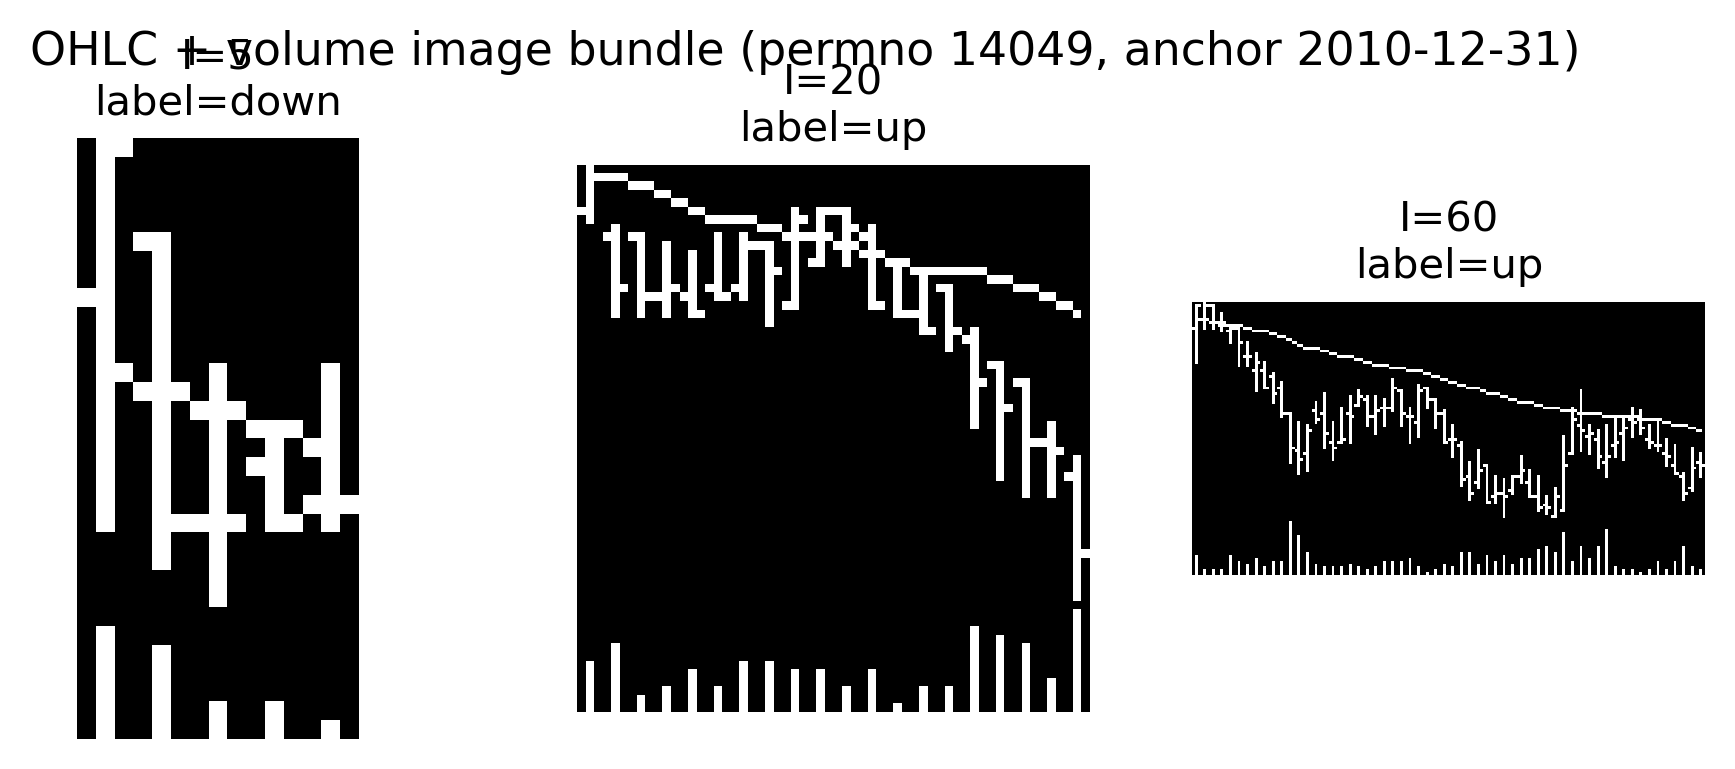
\includegraphics[width=\linewidth]{ohlc_sample.png}
  \caption{OHLC-plus-volume images for a single security at horizons
    $I\in\{5,20,60\}$.}
  \label{fig:ohlc-sample}
\end{figure}

\paragraph{Train/validation/test split.}
We follow the original paper in treating the early portion of
the panel as in-sample. Training is performed on 1993--2000 with a
70/30 random sample-level split for training/validation. Out-of-sample backtests start in January 2001. Headline tables and figures
report results through December 2019, matching the evaluation window in
the original paper.


\section{CNN architecture and training}
\label{sec:arch}

\paragraph{Architectures.}
The three horizon-specific backbones mirror the published configuration.
Each block applies a $5\times3$ convolution, LeakyReLU($0.01$), batch
normalisation, and $2\times1$ max pooling along the time axis. For
$I=20$ and $I=60$, the opening convolution uses dilation and stride to widen
the receptive field without a proportional increase in parameters, and
pooling is configured so that spatial dimensions are preserved enough to
yield the fully connected widths reported in the original paper; the
$I=5$ network is shallower and uses the default pooling rule throughout.
Figure~\ref{fig:cnn-arch} summarises the three stacks; stride, dilation,
and channel widths are listed in Table~\ref{tab:cnn-layers}
(Appendix~\ref{app:hyper}).

\begin{figure}[H]
  \centering
  \resizebox{\linewidth}{!}{%
  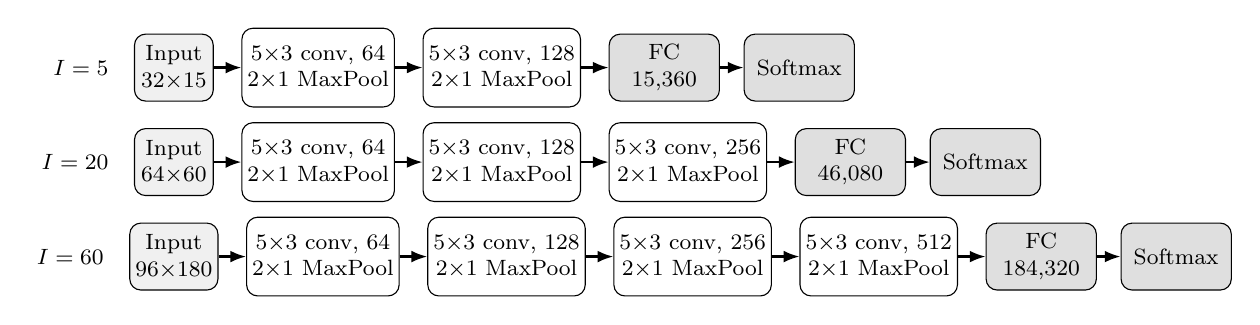
\begin{tikzpicture}[
      font=\footnotesize,
      block/.style={draw, rounded corners, minimum height=1.0cm, minimum width=1.55cm, align=center, inner sep=2pt},
      input/.style={draw, fill=gray!12, rounded corners, minimum height=0.85cm, minimum width=1.0cm, align=center, inner sep=2pt},
      head/.style={draw, fill=gray!25, rounded corners, minimum height=0.85cm, minimum width=1.4cm, align=center, inner sep=2pt},
      arr/.style={-{Latex[length=2mm]}, thick}
    ]
    %% I=5 (two blocks, as in Jiang Figure~2)
    \node[input] (i5in) at (0,2.2) {Input\\$32{\times}15$};
    \node[block, right=3.5mm of i5in] (i5b1) {$5{\times}3$ conv, 64\\$2{\times}1$ MaxPool};
    \node[block, right=3.5mm of i5b1] (i5b2) {$5{\times}3$ conv, 128\\$2{\times}1$ MaxPool};
    \node[head,  right=3.5mm of i5b2] (i5fc) {FC\\15{,}360};
    \node[head,  right=3mm of i5fc] (i5sm) {Softmax};
    \draw[arr] (i5in)  -- (i5b1);
    \draw[arr] (i5b1)  -- (i5b2);
    \draw[arr] (i5b2)  -- (i5fc);
    \draw[arr] (i5fc)  -- (i5sm);
    \node[left=2mm of i5in] {$I=5$};
    %% I=20 (three blocks)
    \node[input] (i20in) at (0,1.0) {Input\\$64{\times}60$};
    \node[block, right=3.5mm of i20in] (i20b1) {$5{\times}3$ conv, 64\\$2{\times}1$ MaxPool};
    \node[block, right=3.5mm of i20b1] (i20b2) {$5{\times}3$ conv, 128\\$2{\times}1$ MaxPool};
    \node[block, right=3.5mm of i20b2] (i20b3) {$5{\times}3$ conv, 256\\$2{\times}1$ MaxPool};
    \node[head,  right=3.5mm of i20b3] (i20fc) {FC\\46{,}080};
    \node[head,  right=3mm of i20fc] (i20sm) {Softmax};
    \draw[arr] (i20in) -- (i20b1);
    \draw[arr] (i20b1) -- (i20b2);
    \draw[arr] (i20b2) -- (i20b3);
    \draw[arr] (i20b3) -- (i20fc);
    \draw[arr] (i20fc) -- (i20sm);
    \node[left=2mm of i20in] {$I=20$};
    %% I=60 (four blocks)
    \node[input] (i60in) at (0,-0.2) {Input\\$96{\times}180$};
    \node[block, right=3.5mm of i60in] (i60b1) {$5{\times}3$ conv, 64\\$2{\times}1$ MaxPool};
    \node[block, right=3.5mm of i60b1] (i60b2) {$5{\times}3$ conv, 128\\$2{\times}1$ MaxPool};
    \node[block, right=3.5mm of i60b2] (i60b3) {$5{\times}3$ conv, 256\\$2{\times}1$ MaxPool};
    \node[block, right=3.5mm of i60b3] (i60b4) {$5{\times}3$ conv, 512\\$2{\times}1$ MaxPool};
    \node[head,  right=3.5mm of i60b4] (i60fc) {FC\\184{,}320};
    \node[head,  right=3mm of i60fc] (i60sm) {Softmax};
    \draw[arr] (i60in) -- (i60b1);
    \draw[arr] (i60b1) -- (i60b2);
    \draw[arr] (i60b2) -- (i60b3);
    \draw[arr] (i60b3) -- (i60b4);
    \draw[arr] (i60b4) -- (i60fc);
    \draw[arr] (i60fc) -- (i60sm);
    \node[left=2mm of i60in] {$I=60$};
  \end{tikzpicture}%
  }
  \caption{Horizon-specific CNN backbones. Each rectangle is one block:
    $5{\times}3$ convolution (with the channel width shown), LeakyReLU,
    batch normalisation, and $2{\times}1$ max pooling. Stride and dilation
    for $I=20$ and $I=60$ are in Table~\ref{tab:cnn-layers}. Fully connected
    input sizes are 15{,}360 ($I=5$), 46{,}080 ($I=20$), and 184{,}320 ($I=60$).}
  \label{fig:cnn-arch}
\end{figure}

\paragraph{Optimisation.}
We minimise binary cross-entropy on the per-horizon label $y_{t,F}$ using
stochastic gradient descent (Adam variant disabled), with learning rate
$10^{-5}$, batch size $128$, and a maximum of $50$ epochs with
early-stopping on validation loss. Convolutional and linear weights are
initialised with Xavier-uniform and biases at zero.

The original paper reports headline results from an ensemble of
independently trained networks whose softmax outputs are averaged at
inference. Our replication proceeded in two stages. For the course
presentation, limited local compute allowed only a single random seed
($42$) per horizon, so we could not yet reproduce the full
ensemble-averaging protocol. For the final project we reran training on
rented cloud GPUs with five seeds
$\{42, 123, 456, 789, 101112\}$ and aggregate by averaging
softmax-probability outputs at inference time, as in the original paper.
All empirical results in Sections~\ref{sec:results}--\ref{sec:saliency}
use this five-seed ensemble. The resulting model sizes are approximately
$0.6$\,MB ($I=5$), $2.8$\,MB ($I=20$), and $11.8$\,MB ($I=60$) per seed,
consistent with the parameter counts implied by Figure~\ref{fig:cnn-arch}.


\section{Empirical results}
\label{sec:results}

We score every test-set observation with the five-seed ensemble and
form ten cross-sectional deciles by predicted ``up''-probability at each
rebalance date. The high-minus-low (H--L) portfolio is equal-weighted
within deciles, rebalanced at horizon-end, and adjusted for proportional
transaction costs at $10$\,bp per side ($20$\,bp round-trip) applied to
both legs.

\subsection{Cross-sectional deciles versus conventional benchmarks}
\label{sec:deciles}

Our first empirical object is unconditional decile-sort performance. At
each horizon $I\in\{5,20,60\}$ we partition stocks into predicted-probability
deciles using the CNN ensemble score, and we form analogous deciles from
matched-horizon momentum, moving-average crossover, and short-term reversal
signals constructed on the same out-of-sample panel and rebalance calendar.
For every horizon we summarise average annualised realised \emph{levels} and
volatilities by decile in the dual-panel layout of Figure~7 in the original
paper (returns on the left, volatilities on the right), overlaying all four
signals to contrast the CNN's ranking with traditional patterns. To keep the
main exposition readable, Figure~\ref{fig:fig7} reports only the $I=5$
(weekly) case, which is also where the economic spread survives costs most
clearly; Appendix~\ref{app:fig7-horizons} reproduces the identical format for
$I=20$ and $I=60$.

\begin{figure}[H]
  \centering
  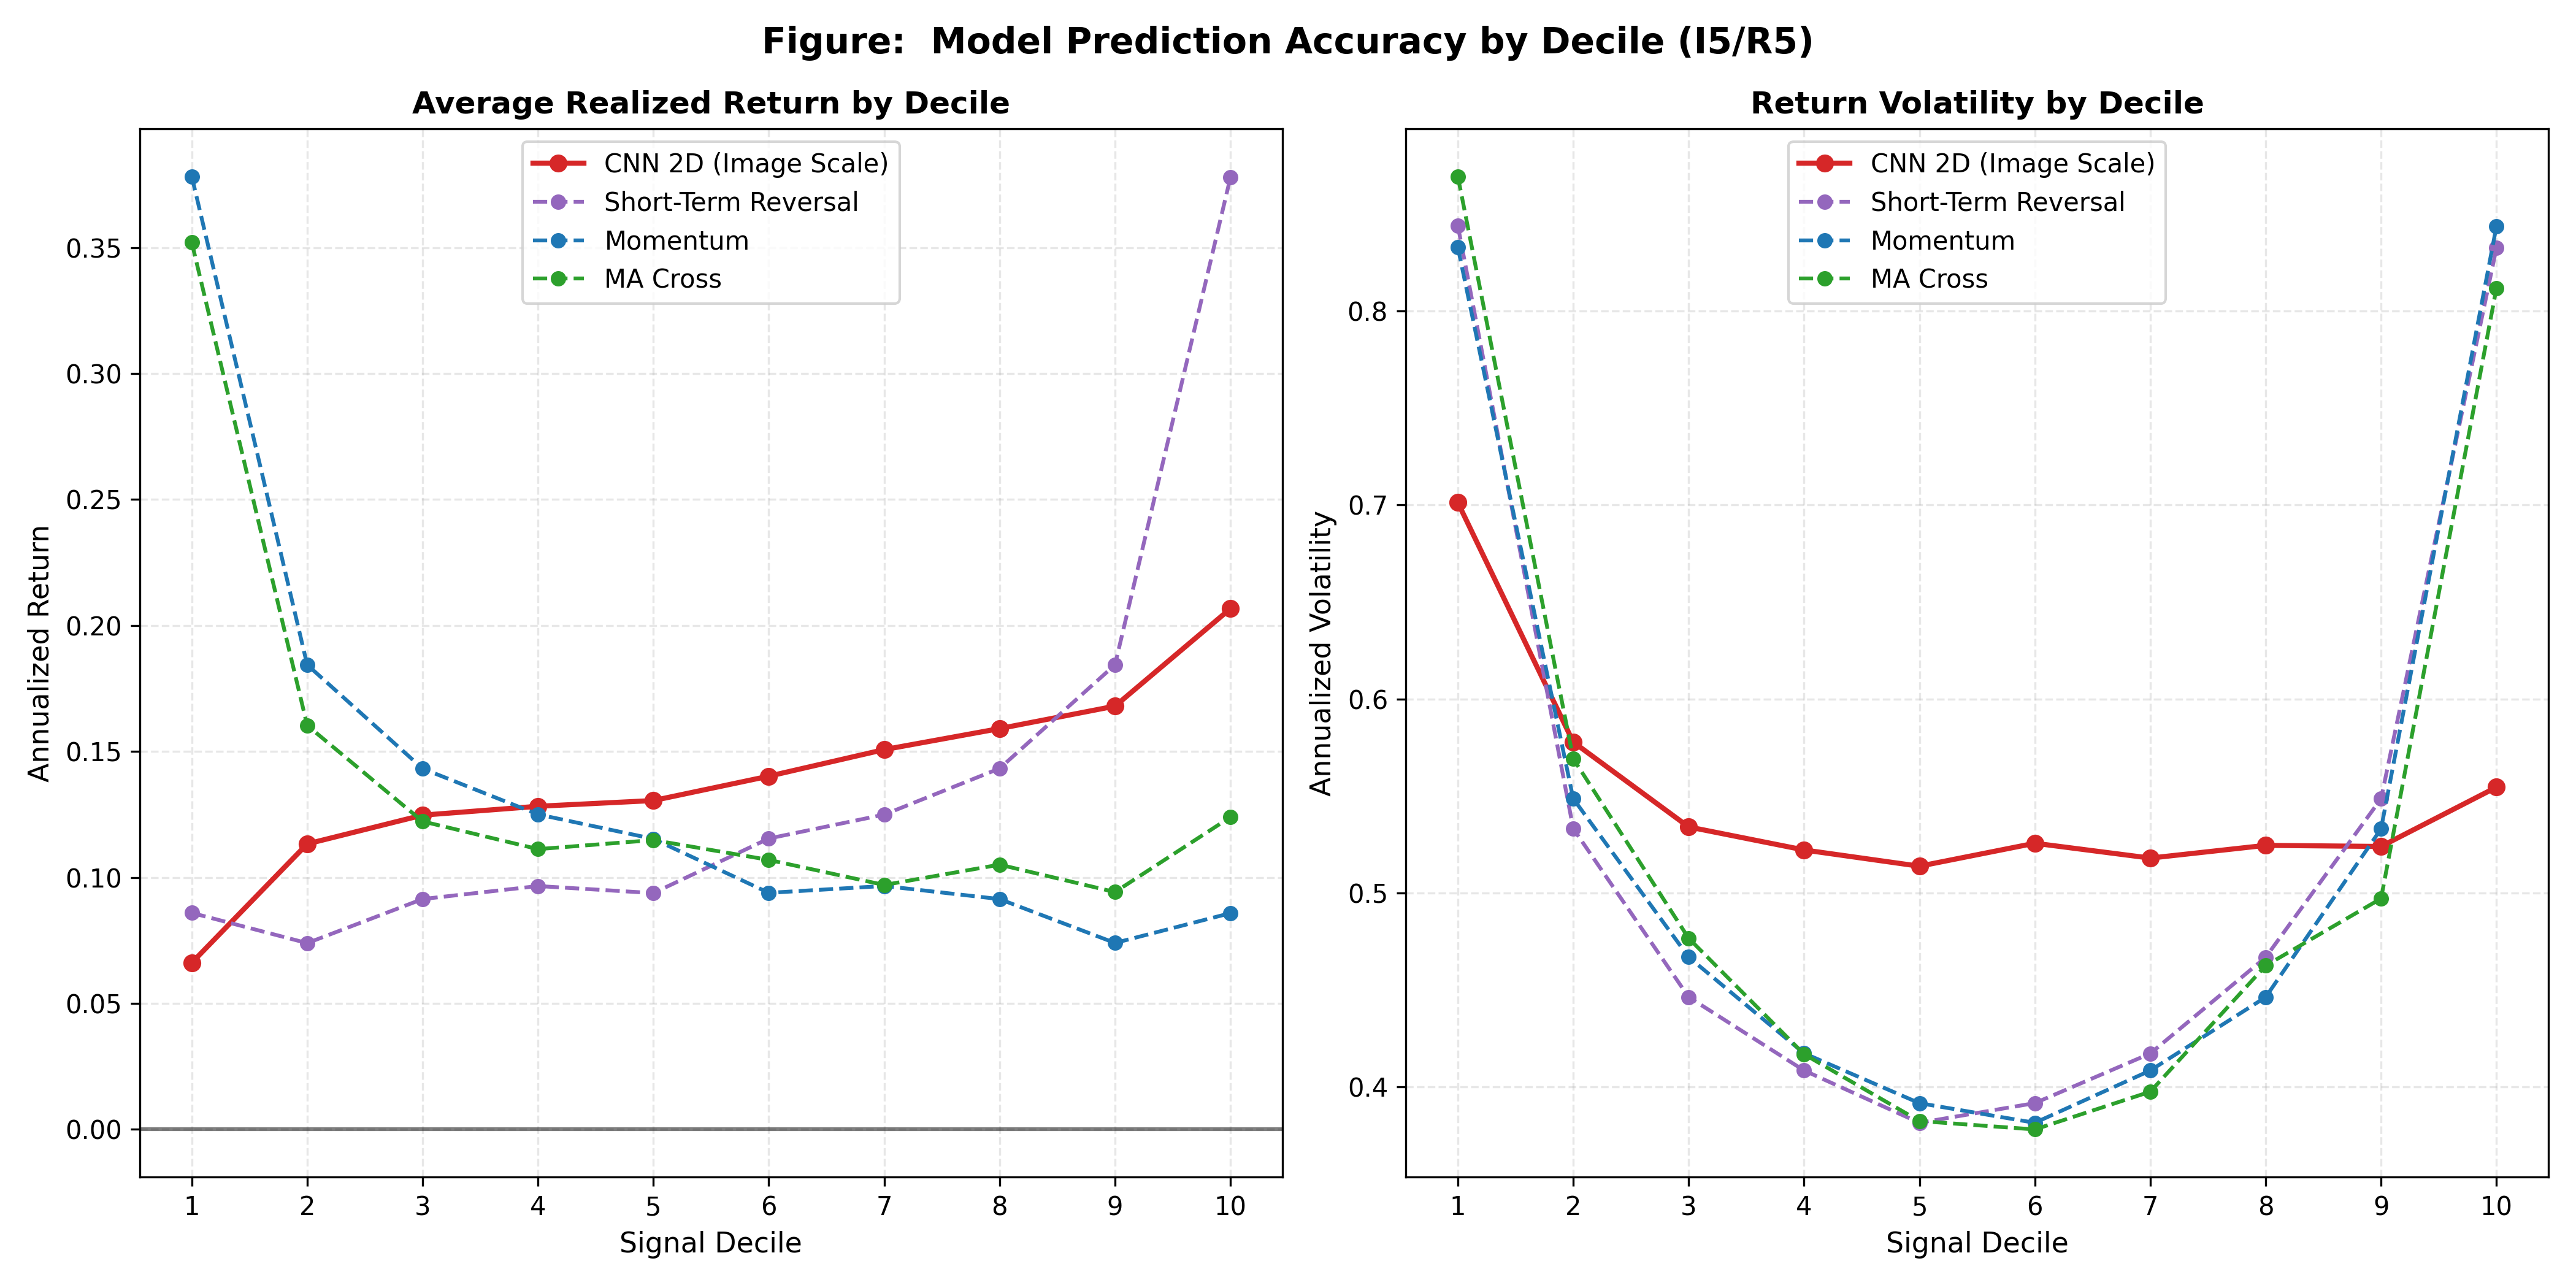
\includegraphics[width=0.82\linewidth]{fig7_I5.png}
  \caption{CNN deciles against momentum, moving-average cross, and
    short-term reversal baselines at the $I=5$ horizon. Reproduction of
    Figure~7 of the original paper. The reversal baseline's D10 reaches an
    annualised return of $37.78\%$, against which the CNN's monotone ranking
    is more useful as a cross-sectional signal than as a stand-alone
    strategy. Analogous plots for $I=20$ and $I=60$ are in
    Appendix~\ref{app:fig7-horizons}.}
  \label{fig:fig7}
\end{figure}

At $I=5$, the CNN traces a stable, nearly monotone gradient across
deciles---annualised realised returns rise from $6.62\%$ in D1 to
$20.67\%$ in D10---so predicted probability cleanly orders the cross-section,
which is precisely what portfolio construction needs when translating a scalar
forecast into decile-ranked positions. Matched-horizon momentum and
moving-average signals, by contrast, show little separation across deciles:
their profiles remain comparatively flat between D1 and D10, implying weak
incremental discriminatory power rather than an economically coherent
ranking ladder. Figure~\ref{fig:fig7} therefore highlights how the CNN
systematically aligns predicted ``up'' probability with realised performance

The short-term reversal line offers a contrasting story: isolated tail
positions can deliver very high average returns (notably around
$37.78\%$ at extreme deciles tied to battered names and bounce effects), yet
those readings are intermittent and mechanically concentrated rather than part
of a smooth cross-sectional map. Relative to reversal, then, the CNN is the
most reliable vehicle for exploiting the chart-based signal globally across
every decile, which is why it remains the cornerstone of our long--short
construction even though naive reversal exposures can episodically post larger
average returns.

At longer horizons---Appendix Figures~\ref{fig:fig7-i20} and~\ref{fig:fig7-i60}
---the classical benchmarks become structurally uneven: momentum and MA both
bend into pronounced U-shaped patterns, with dispersion jumping at the extremes
rather than drifting steadily with the sorting variable; that curvature is less
investable for uniform decile-spanning mandates and aligns with intermittent
premium pockets rather than a stable scoring rule. Against this backdrop the
CNN's decile trajectory remains comparatively smooth across the histogram: even
when the D10-vs-D1 wedge narrows (e.g.\ $11.10\%$ vs.\ $9.78\%$ at $I=20$, or an
approximately flat footprint at $I=60$), the CNN seldom exhibits the bipolar
bounce between bottom and top deciles that dominates the plotted traditional
signals, underscoring the relative stability with which convolutional summaries
preserve a coherent monotone ordering versus ad hoc extremes of reversal and
price-trend heuristics.


\subsection{Short-horizon portfolio performance}

Image-based forecasts are most useful economically if they translate into
profitable portfolios, not merely higher classification scores. Following the
short-horizon portfolio analysis in the original paper, we therefore focus first
on the weekly signal and ask whether the CNN ranking produces persistent
long--short gains relative to standard price-trend benchmarks. The portfolio
return is the gross high-minus-low spread between the top and bottom forecast
deciles. Equal-weighted and value-weighted CNN spreads are shown separately,
and the weekly momentum and moving-average spreads are constructed on the same
rebalance calendar.

One implementation choice differs from the original paper. Its Figure~5 uses a
common weekly holding period for several image lengths, whereas our portfolio
backtests use matched prediction and holding horizons: $I=5$ is rebalanced every
five trading days, $I=20$ every 20 trading days, and $I=60$ every 60 trading
days. We adopt this design because the trained labels, forecast panels, and
transaction-cost calculations in this replication are horizon matched
($F=I$). It avoids applying a 20- or 60-day image model to a weekly trading
problem for which it was not trained, and it makes turnover and holding-period
returns internally comparable across the reported tables and figures.

Figure~\ref{fig:fig8} reports cumulative \emph{volatility-adjusted} log
returns. For a strategy with periodic gross spread $r_t^{s}$, and a benchmark
holding-period return $r_t^{b}$ measured over the same interval, we compute
\[
  \tilde r_t^{s}
  =
  r_t^{s}
  \frac{\sigma_b}{\sigma_s},
\]
where $\sigma_s$ and $\sigma_b$ are the full-sample standard deviations of the
strategy and benchmark returns on their common dates. The plotted series is
$\sum_t \log(1+\tilde r_t^{s})$. This normalization puts all strategies on the
same volatility scale as the equity benchmark, so differences in slope reflect
average return per unit of matched risk rather than mechanical differences in
unconditional volatility.\footnote{The benchmark is SPY when the data download
succeeds and the Fama--French cash-inclusive daily market otherwise. The
$I=20$ and $I=60$ CNN lines use our cached monthly and quarterly native
rebalancing calendars, labelled I20/R20 and I60/R60. Thus those two lines are
included as longer-horizon diagnostics rather than exact replicas of the
original paper's common weekly-holding overlays.}

\begin{figure}[H]
  \centering
  
\includegraphics[width=\linewidth]{figure5_vol_adjusted_cumlog.png}
  \caption{Cumulative volatility-adjusted log returns of gross long--short
    portfolios. Each strategy is rescaled to the volatility of the benchmark
    measured over the same holding intervals; no transaction costs are applied
    in this figure.}
  \label{fig:fig8}
\end{figure}

The figure supports the central economic message of the reproduction. On the
weekly calendar, the CNN long--short portfolios accumulate substantially more
volatility-adjusted return than the momentum and moving-average benchmarks. The
equal-weighted CNN curve is especially strong, while the value-weighted version
also remains above the traditional trend signals for most of the evaluation
window. In contrast, momentum and moving-average spreads contribute little
sustained growth after volatility matching, which is consistent with the
decile evidence in Figure~\ref{fig:fig7}: scalar trend rules do not generate
as stable a cross-sectional ordering as the image-based CNN score.

The longer-horizon CNN curves are flatter, which mirrors the weaker decile
separation at $I=20$ and $I=60$. This does not contradict the short-horizon
result. Rather, it suggests that the strongest economic content of the chart
representation is concentrated in recent price and volume patterns. Because
Figure~\ref{fig:fig8} is gross of transaction costs, it should be read together with
Table~\ref{tab:table1}: once turnover and transaction costs are applied, only
the weekly CNN spread retains a robust net Sharpe ratio.

\subsection{Decile portfolio statistics}

\begin{table}[t]
  \centering
  \caption{Equal-weighted decile portfolio statistics (reproduction of
    Table~1 in the original paper).
    \texttt{Ret} is annualised mean return, \texttt{Std} annualised standard
    deviation, \texttt{SR} the resulting Sharpe ratio. ``H--L'' columns
    are for the long--short decile spread net of $20$\,bp round-trip
    transaction costs.}
  \label{tab:table1}
  \small
  \begin{tabular}{l rrrrrrrrrrr r}
    \toprule
       & D1 & D2 & D3 & D4 & D5 & D6 & D7 & D8 & D9 & D10 & H--L \\
    \midrule
    \multicolumn{12}{l}{\textbf{$I=5$ (weekly rebalance, turnover $0.858$)}}\\
    Ret & 0.07 & 0.12 & 0.13 & 0.13 & 0.14 & 0.15 & 0.16 & 0.16 & 0.17 & 0.21 & 0.14 \\
    Std & 0.13 & 0.16 & 0.17 & 0.17 & 0.18 & 0.18 & 0.19 & 0.19 & 0.20 & 0.21 & 0.11 \\
    SR  & 0.55 & 0.75 & 0.77 & 0.77 & 0.75 & 0.79 & 0.83 & 0.85 & 0.89 & 1.04 & 1.29 \\
    \midrule
    \multicolumn{12}{l}{\textbf{$I=20$ (monthly rebalance, turnover $0.841$)}}\\
    Ret & 0.10 & 0.12 & 0.13 & 0.12 & 0.11 & 0.12 & 0.11 & 0.11 & 0.11 & 0.11 & 0.01 \\
    Std & 0.17 & 0.18 & 0.18 & 0.18 & 0.18 & 0.18 & 0.17 & 0.17 & 0.17 & 0.17 & 0.08 \\
    SR  & 0.59 & 0.63 & 0.72 & 0.65 & 0.63 & 0.65 & 0.65 & 0.66 & 0.68 & 0.68 & 0.16 \\
    \midrule
    \multicolumn{12}{l}{\textbf{$I=60$ (quarterly rebalance, turnover $0.867$)}}\\
    Ret & 0.13 & 0.13 & 0.13 & 0.14 & 0.13 & 0.12 & 0.13 & 0.13 & 0.12 & 0.12 & $-0.01$ \\
    Std & 0.22 & 0.20 & 0.20 & 0.19 & 0.20 & 0.19 & 0.18 & 0.18 & 0.17 & 0.16 & 0.11 \\
    SR  & 0.60 & 0.65 & 0.67 & 0.71 & 0.65 & 0.67 & 0.69 & 0.73 & 0.73 & 0.77 & $-0.11$ \\
    \bottomrule
  \end{tabular}
\end{table}

Table~\ref{tab:table1} confirms what Figure~\ref{fig:fig7} shows in cross-section together with Figure~\ref{fig:fig8} (risk-matched gross time series): only the $I=5$
horizon delivers a
robust net H--L spread (annualised SR $1.29$). At $I=20$ the H--L SR is
$0.16$, and at $I=60$ the spread is mildly negative ($-0.11$). The
monotone increase in within-decile Sharpe ratios at $I=60$ (from $0.60$
at D1 to $0.77$ at D10) shows that the CNN \emph{ordering} is still
informative, but the gross spread is too small relative to volatility to
survive transaction costs.

\subsection{Classification metrics}

\begin{table}[t]
  \centering
  \caption{Out-of-sample binary classification metrics for the CNN
    ensemble (2001--2019). $N_{\mathrm{test}}$ is the number of rebalance-day
    observations scored by the five-seed ensemble.}
  \label{tab:classmetrics}
  \small
  \begin{tabular}{lrrr}
    \toprule
    Horizon & Accuracy & AUC--ROC & $N_{\mathrm{test}}$ \\
    \midrule
    $I=5$  & 49.45\% & 0.5103 & 6{,}378{,}408 \\
    $I=20$ & 52.68\% & 0.5242 & 1{,}441{,}167 \\
    $I=60$ & 53.70\% & 0.5288 & ~~~453{,}847 \\
    \bottomrule
  \end{tabular}
\end{table}

Table~\ref{tab:classmetrics} shows that AUC rises with horizon, in line
with the original paper, which argues that longer
look-back windows expose more learnable structure; accuracy at $I=5$ is
\emph{below} the $50\%$ benchmark, which is consistent with a left-skewed
label distribution (more days lose money in the weekly rebalance
universe) rather than a strictly negative signal: the H--L Sharpe of
$1.29$ shows that the predicted-probability \emph{ranking} is far more
informative than the binary forecast.

\subsection{Fama--French five-factor + momentum spanning}

\begin{table}[t]
  \centering
  \caption{Fama--French five-factor plus momentum spanning regressions for
    the net CNN long--short spread. The dependent variable is
    $r_t^{\mathrm{CNN,LS}}-r_t^f$ regressed on
    $\{$Mkt--RF, SMB, HML, RMW, CMA, Mom$\}$ at the matched rebalance
    frequency. Alphas are annualised; $t$-statistics are in parentheses.}
  \label{tab:ff6}
  \small
  \begin{tabular}{lccc}
    \toprule
                          & $I=5$ & $I=20$ & $I=60$ \\
    \midrule
    $\alpha$ (annualised, \%) & $+0.28$  & $-4.30$ & $-6.65$ \\
                              & $(0.13)$ & $(-2.23)$ & $(-3.77)$ \\
    $\beta_{\mathrm{Mkt-RF}}$ & $0.29$ $(14.24)$ & $0.10$ $(2.21)$ & $0.08$ $(1.24)$ \\
    $\beta_{\mathrm{SMB}}$    & $0.14$ $(3.81)$  & $0.01$ $(0.11)$ & $-0.14$ $(-1.24)$ \\
    $\beta_{\mathrm{HML}}$    & $0.13$ $(3.57)$  & $0.02$ $(0.27)$ & $0.23$ $(2.21)$ \\
    $\beta_{\mathrm{RMW}}$    & $0.02$ $(0.41)$  & $0.32$ $(3.48)$ & $0.69$ $(5.24)$ \\
    $\beta_{\mathrm{CMA}}$    & $-0.25$ $(-4.20)$ & $-0.11$ $(-0.98)$ & $-0.29$ $(-2.01)$ \\
    $\beta_{\mathrm{Mom}}$    & $-0.03$ $(-1.51)$ & $-0.00$ $(-0.05)$ & $0.23$ $(3.86)$ \\
    $R^{2}$                   & 0.34 & 0.07 & 0.63 \\
    $N$ periods               & 989  & 226  & 74   \\
    \bottomrule
  \end{tabular}
\end{table}

The regression in Table~\ref{tab:ff6} delivers three messages. First, at
$I=5$ the strategy's annualised alpha is statistically indistinguishable
from zero ($+0.28\%$, $t=0.13$): the high raw Sharpe is largely captured
by factor exposures (significant loadings on Mkt--RF, SMB, HML, and an
opposite-signed load on CMA). Second, at $I=20$ and $I=60$ the alphas
are \emph{negative} and significant ($-4.30\%$, $t=-2.23$; $-6.65\%$,
$t=-3.77$); the loadings on RMW are positive and large, and at $I=60$ the
strategy also picks up a positive momentum loading. Third, the very
high $R^{2}$ at $I=60$ ($0.63$) suggests that the CNN signal at this
horizon is essentially a re-weighting of standard style factors rather
than an independent source of premia.


\section{Interpretability: input-gradient saliency}
\label{sec:saliency}

\begin{figure}[t]
  \centering
  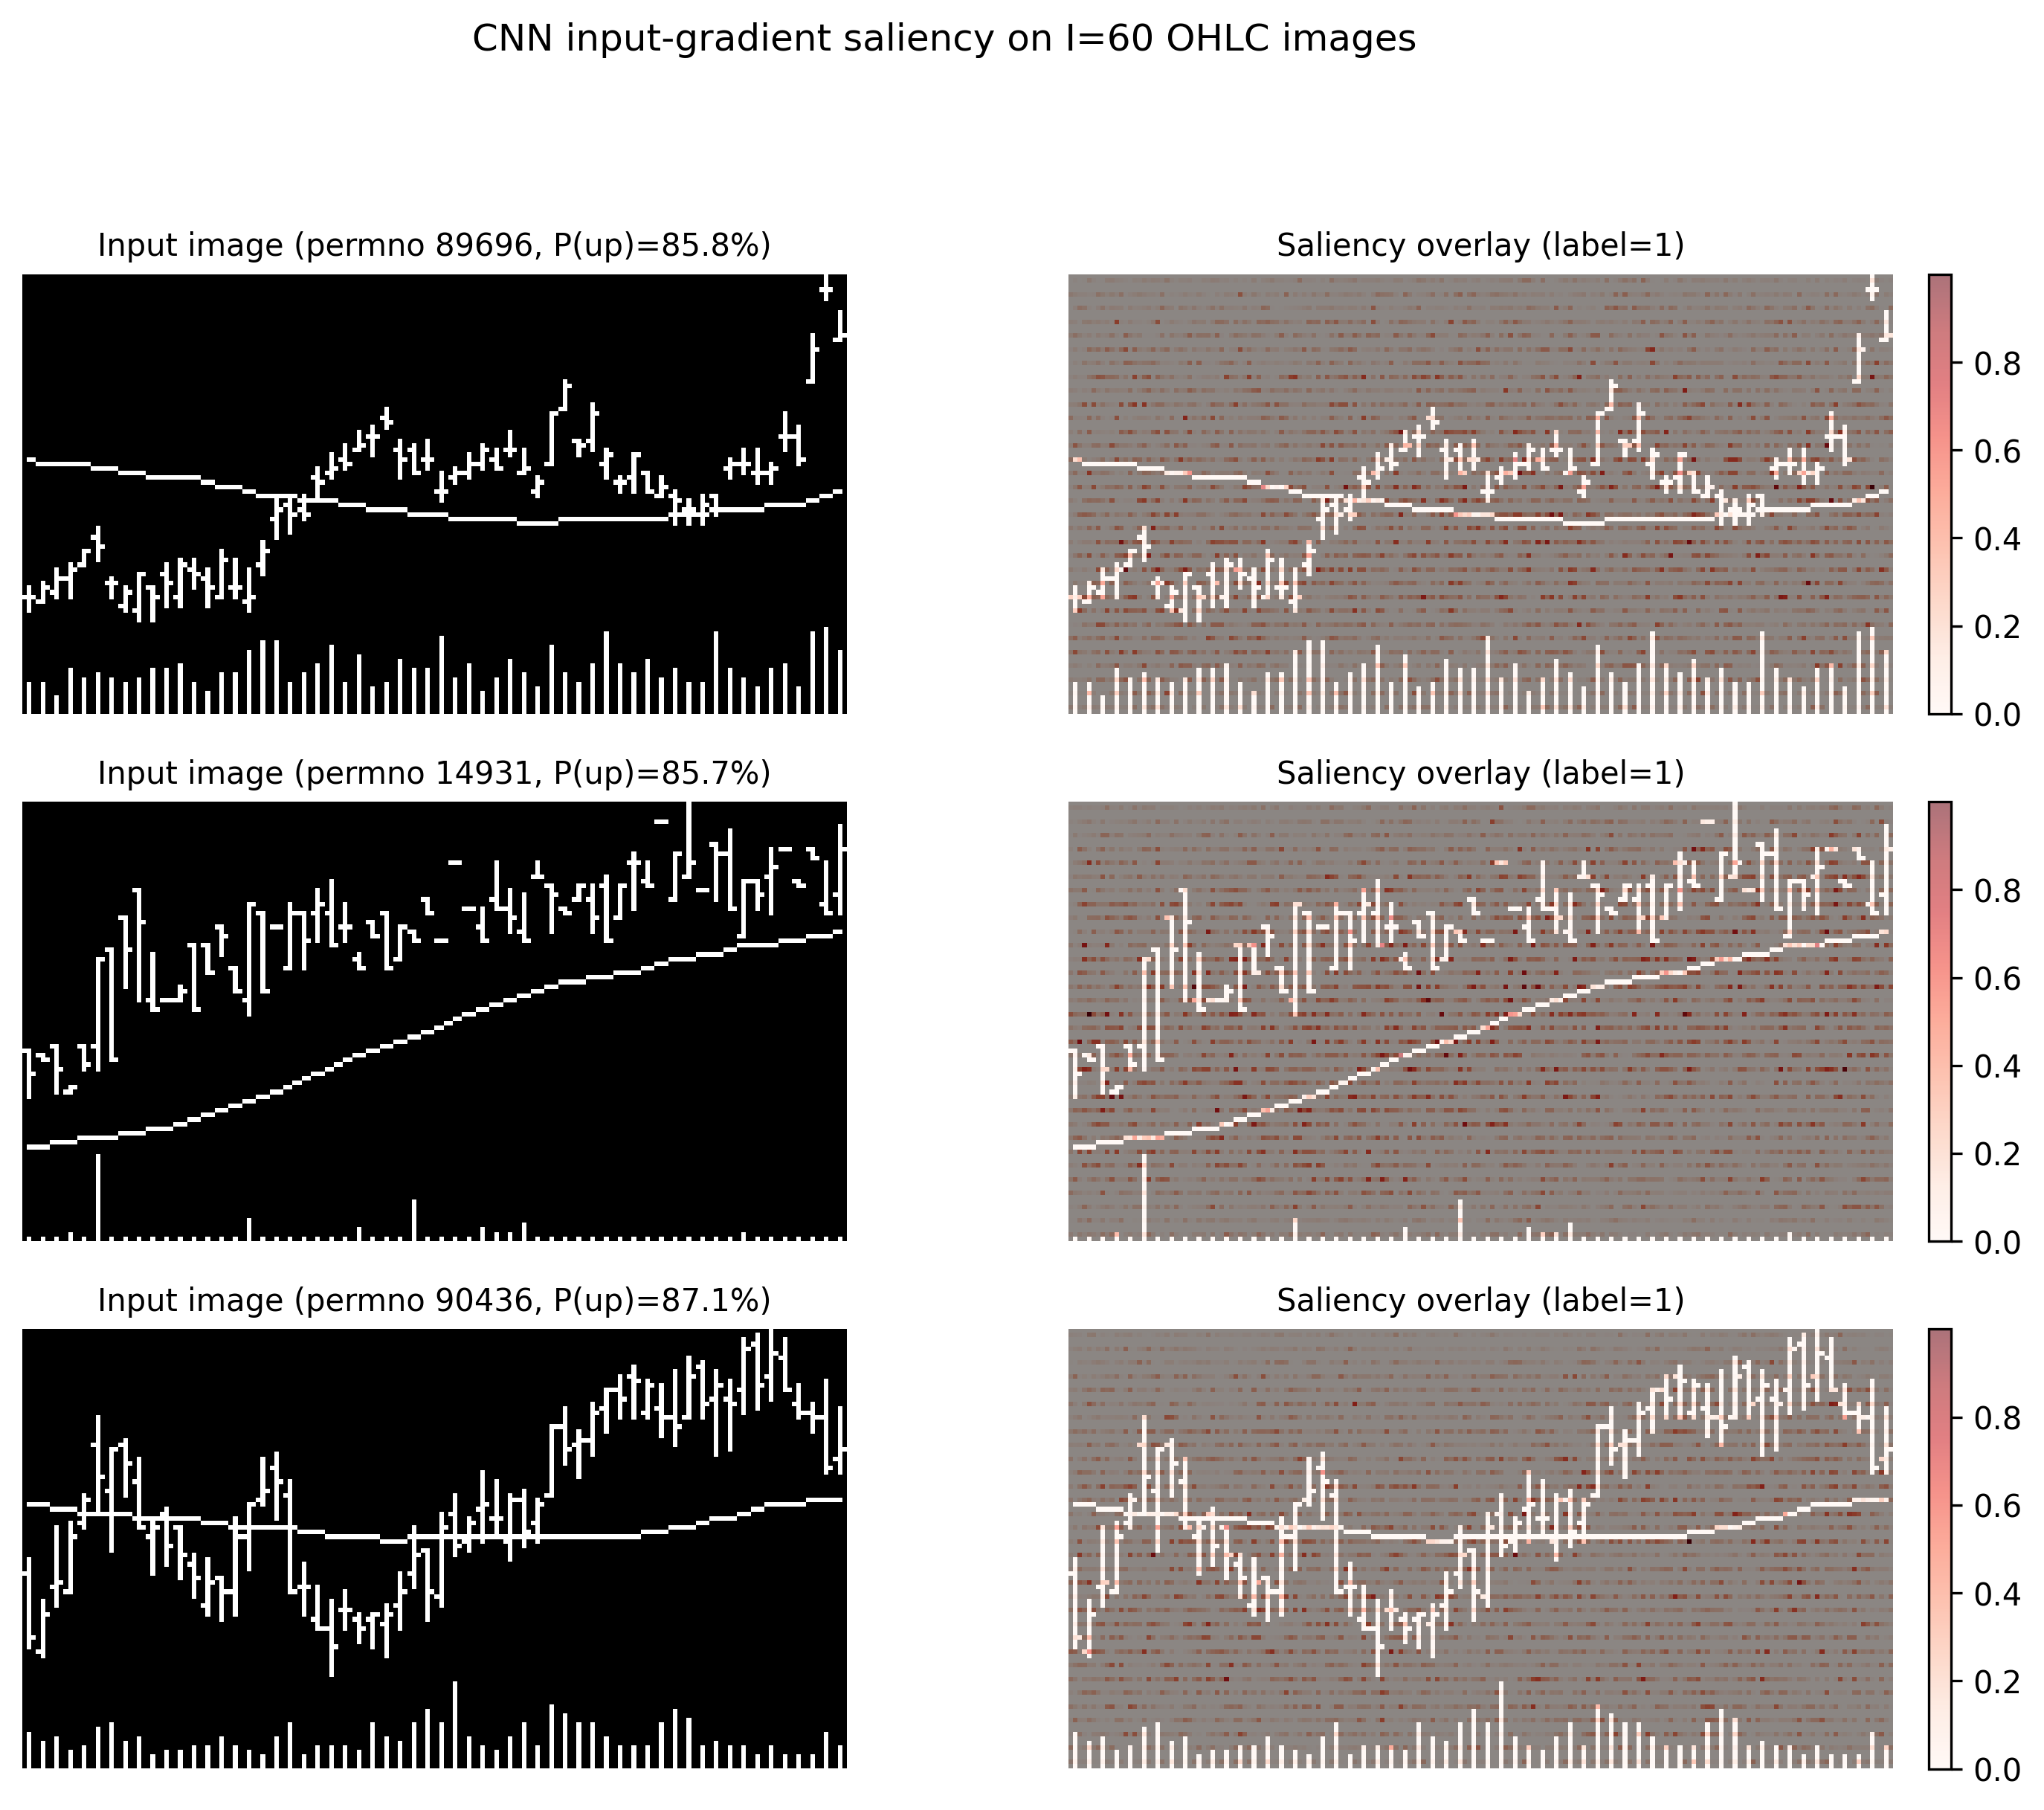
\includegraphics[width=\linewidth]{saliency_I60.png}
  \caption{Input-gradient saliency for three high-confidence positive
    predictions of the $I=60$ ensemble. Left column: the input chart
    (inverted to a white background for readability). Right
    column: the same image with the gradient magnitude $|\partial f_{\text{up}}/\partial x|$
    overlaid in red. The network's attention concentrates on the
    right-most third of each window (i.e.\ the most-recent price action)
    and on volume bars near regime changes.}
  \label{fig:saliency}
\end{figure}

Following \citet{simonyan2014deep}, we compute the absolute pixel-level
gradient of the ``up'' logit with respect to each input image for three
high-confidence positive examples drawn from the $I=60$ test window
(Figure~\ref{fig:saliency}). Across all three examples the saliency mass
is concentrated on the right-most $10$--$20\%$ of the OHLC panel and on
volume bars near sharp price moves. This is consistent with a
data-driven momentum reading: the CNN essentially learns to up-weight
the most-recent observations, which is also the regime in which classical
price-trend signals concentrate their power.


\section{Discussion and conclusion}
\label{sec:discussion}

We recover the qualitative shape of
the original paper at $I=5$ -- a monotone decile ranking, a
high gross-of-cost H--L spread that survives transaction costs into a
$1.29$ net Sharpe ratio, and a decile-by-decile dominance over momentum
and moving-average cross. At $I=20$ and $I=60$ the qualitative ranking
is preserved (Table~\ref{tab:table1}, Figure~\ref{fig:fig7}), but the
H--L spread is too thin to survive costs, and the Fama--French six-factor
regression delivers a statistically significant \emph{negative} alpha at
both horizons.

Several factors plausibly account for numerical differences relative to
the original paper. (i) Our CRSP-style extract, liquidity filters,
and ETF-based calendar construction need not coincide exactly with the original paper's.
(ii) We aggregate five randomly seeded models; the original paper's headline results pool
a larger ensemble, which can stabilise probability estimates. (iii) Small
implementation choices---chart rasterisation, float rounding, and how
turnover maps into proportional costs---can move Sharpe ratios and alphas
when gross spreads are thin.

The saliency analysis (Figure~\ref{fig:saliency}) shows that the
$I=60$ CNN learns a momentum-like reading rather than a more exotic
pattern; this is consistent with a model whose alpha is largely
spanned by RMW and Mom. Promising directions for future work include
regime-conditioned heads, industry- or size-neutralised label
construction, and a mixture-of-experts ensemble that explicitly
allocates capacity across horizons.


\bibliographystyle{plainnat}
\bibliography{references}


\appendix

\section{Reproduction artefact map}
\label{app:artefacts}

Every numerical claim in this paper traces back to a file in
\texttt{final\_submit\_version/outputs/}:
\begin{itemize}
  \item Figure~\ref{fig:ohlc-sample}: produced by
        \texttt{scripts/pipeline\_split/export\_paper\_assets.py}.
  \item Figure~\ref{fig:fig7} (appendix Figures~\ref{fig:fig7-i20} and
        \ref{fig:fig7-i60}): PNGs in
        \texttt{pipeline\_runs/figures/}; decile-level CSVs via
        \texttt{fig7\_simple\_I\{5,20,60\}\_*.csv} (the pipeline additionally
        exports Figure~6-style tables for reproducibility auditing).
  \item Figure~\ref{fig:fig8}:
        \texttt{pipeline\_runs/figures/figure5\_vol\_adjusted\_cumlog.png}
        produced by \texttt{scripts/pipeline\_split/plot\_figure5\_vol\_adjusted\_cumlog.py}
        from cached \texttt{backtest\_I\{5,20,60\}.pkl} and a downloaded equity benchmark;
        optional auxiliary six-panel grids remain in \texttt{ppt\_images/ppt15\_cumulative\_returns*.png}.
  \item Table~\ref{tab:table1}:
        \texttt{pipeline\_runs/tables/table1\_I\{5,20,60\}.csv}.
  \item Table~\ref{tab:classmetrics}:
        \texttt{ppt\_images/ppt16\_classification\_metrics.csv} plus
        shape of \texttt{cache/preds\_I\{5,20,60\}.npy}.
  \item Table~\ref{tab:ff6}: produced by
        \texttt{scripts/pipeline\_split/export\_ff\_regression.py};
        intermediate file
        \texttt{pipeline\_runs/tables/ff\_regression\_combined.csv}.
  \item Figure~\ref{fig:saliency}: produced by
        \texttt{scripts/pipeline\_split/export\_saliency\_map.py} using
        the $I=60$ checkpoint at seed $42$.
\end{itemize}

\section{Hyperparameters and per-block tensor shapes}
\label{app:hyper}

Table~\ref{tab:cnn-layers} reports the per-block configuration used in
the three CNN backbones; all blocks share the
Conv$\to$BatchNorm$\to$LeakyReLU($0.01$)$\to$MaxPool$(2,1)$ pattern.

\begin{table}[h]
  \centering
  \caption{CNN backbone configuration by horizon. ``--'' denotes a
    convolutional block not used for that horizon. FC input dimensions match
    Figure~\ref{fig:cnn-arch}.}
  \label{tab:cnn-layers}
  \small
  \begin{tabular}{lccc}
    \toprule
    Block & $I=5$ & $I=20$ & $I=60$ \\
    \midrule
    Block 1 channels    & $1\to64$ & $1\to64$ & $1\to64$ \\
    Block 1 stride      & (1,1) & (3,1) & (3,1) \\
    Block 1 dilation    & (1,1) & (2,1) & (3,1) \\
    Block 2 channels    & $64\to128$ & $64\to128$ & $64\to128$ \\
    Block 3 channels    & --         & $128\to256$ & $128\to256$ \\
    Block 4 channels    & --         & --          & $256\to512$ \\
    FC input dim        & 15{,}360 & 46{,}080    & 184{,}320 \\
    Approx.\ params     & $\sim$\,150\,k & $\sim$\,700\,k & $\sim$\,3.0\,M \\
    \bottomrule
  \end{tabular}
\end{table}

\section{Computational footprint}
\label{app:compute}

The cleaned daily panel occupies approximately $11.1$\,GB. Per-seed model
checkpoints are approximately $0.6$\,MB ($I=5$), $2.8$\,MB ($I=20$), and
$11.8$\,MB ($I=60$); five seeds per horizon give a total of about $76$\,MB.
Training and ensemble inference were performed on a single CUDA GPU (with
an Apple-silicon fallback for development); end-to-end execution of the
pipeline takes on the order of a few wall-clock hours once the cleaned panel
has been constructed.


\section{Baseline comparison plots for \texorpdfstring{$I=20$}{I=20} and \texorpdfstring{$I=60$}{I=60}}
\label{app:fig7-horizons}

\begin{figure}[H]
  \centering
  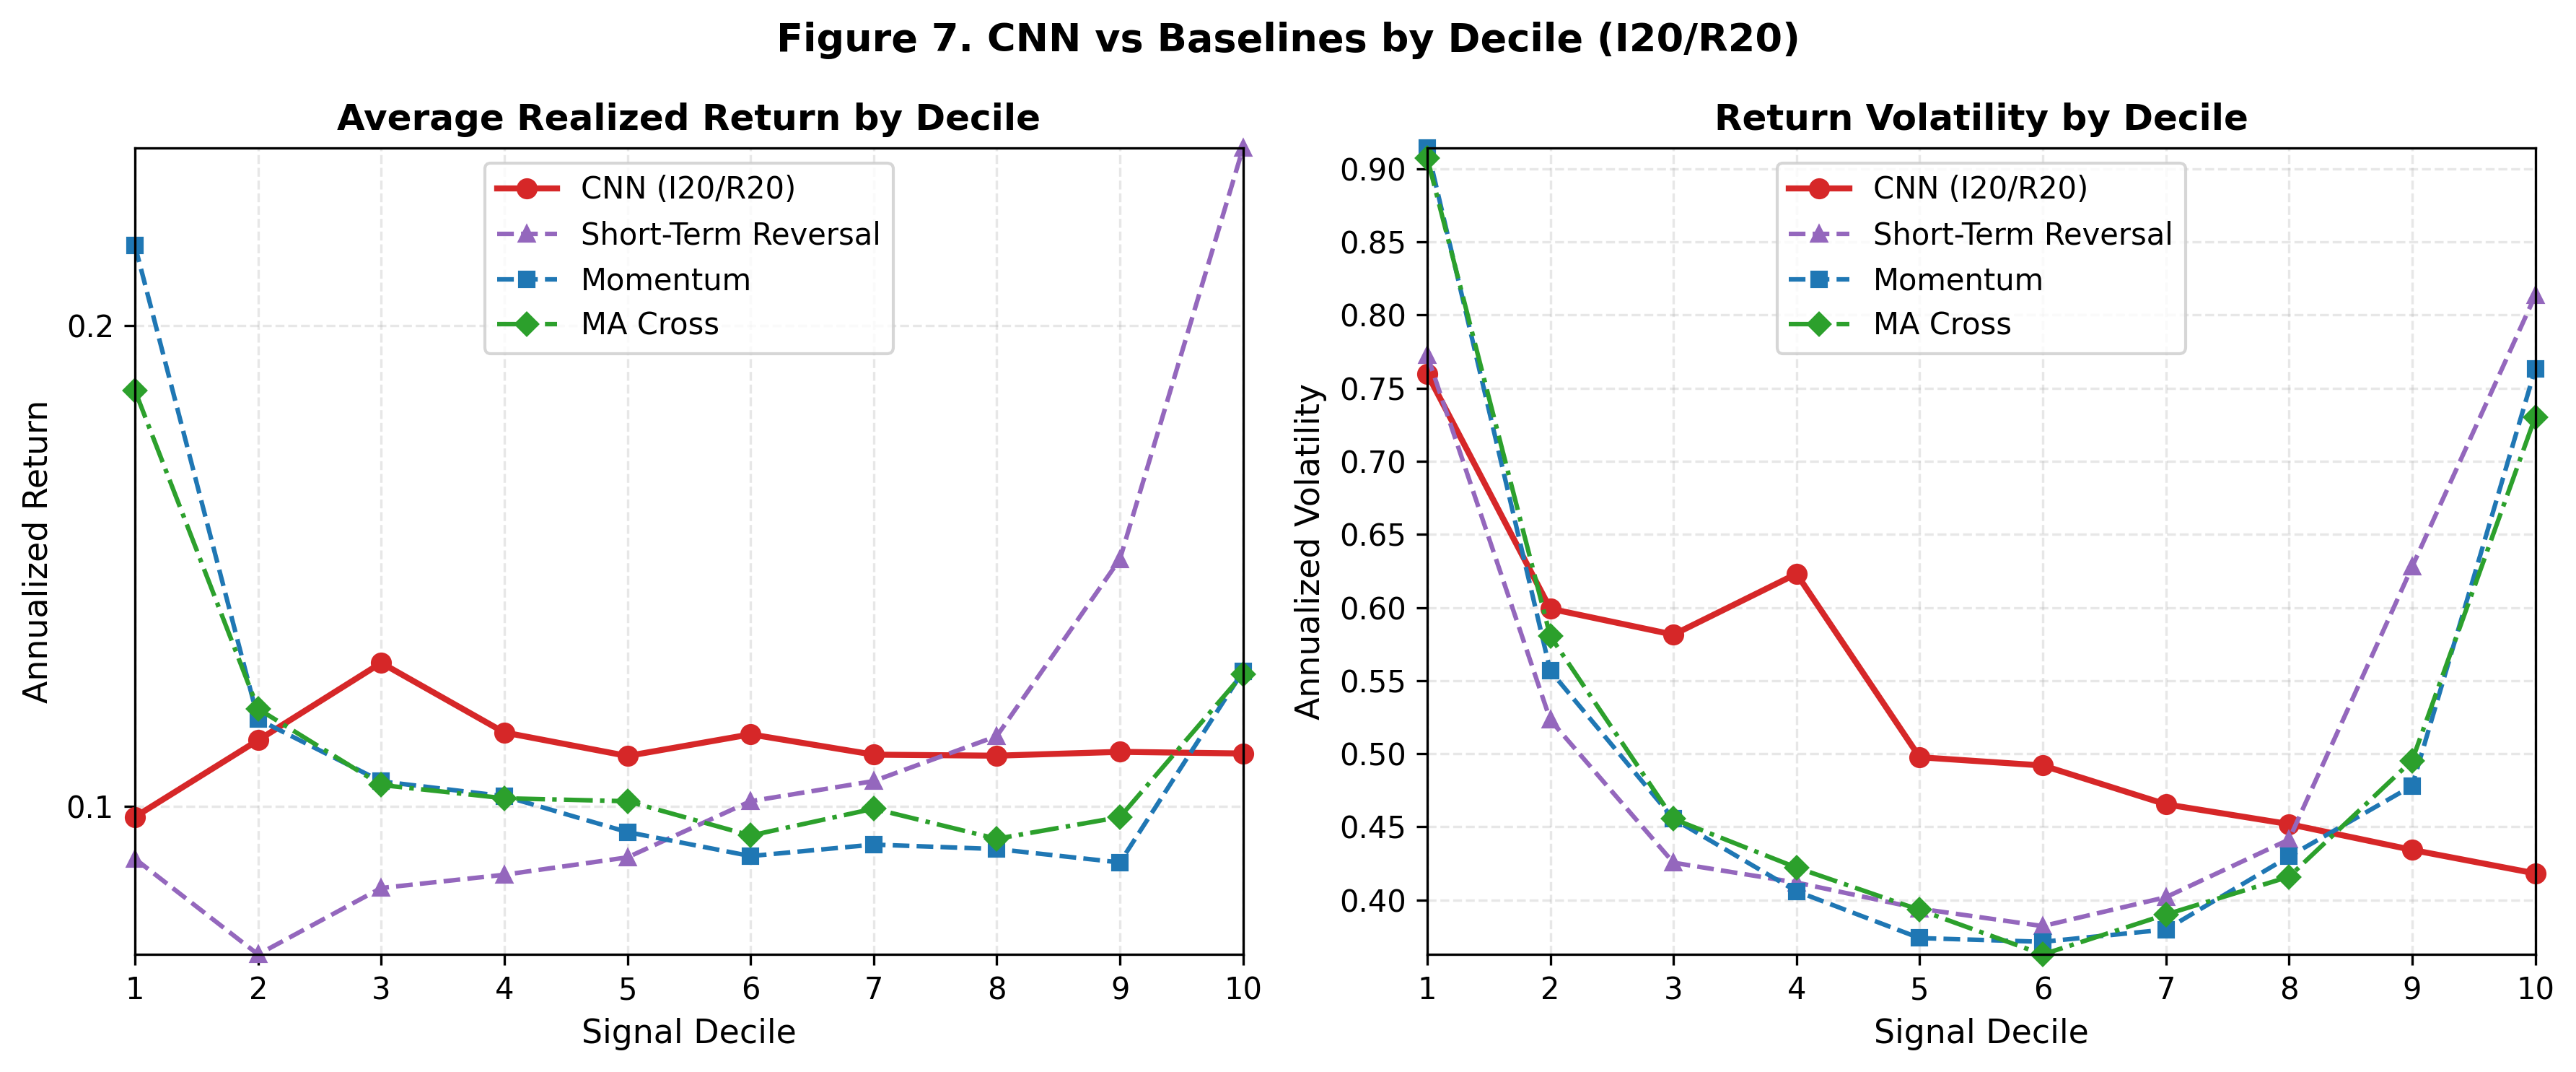
\includegraphics[width=0.82\linewidth]{fig7_I20.png}
  \caption{CNN deciles against momentum, moving-average cross, and
    short-term reversal baselines at the $I=20$ horizon. Reproduction of
    Figure~7 of the original paper. The CNN's monotone ranking is
    qualitatively closer to the monthly-frequency pattern than at $I=5$.}
  \label{fig:fig7-i20}
\end{figure}

\begin{figure}[H]
  \centering
  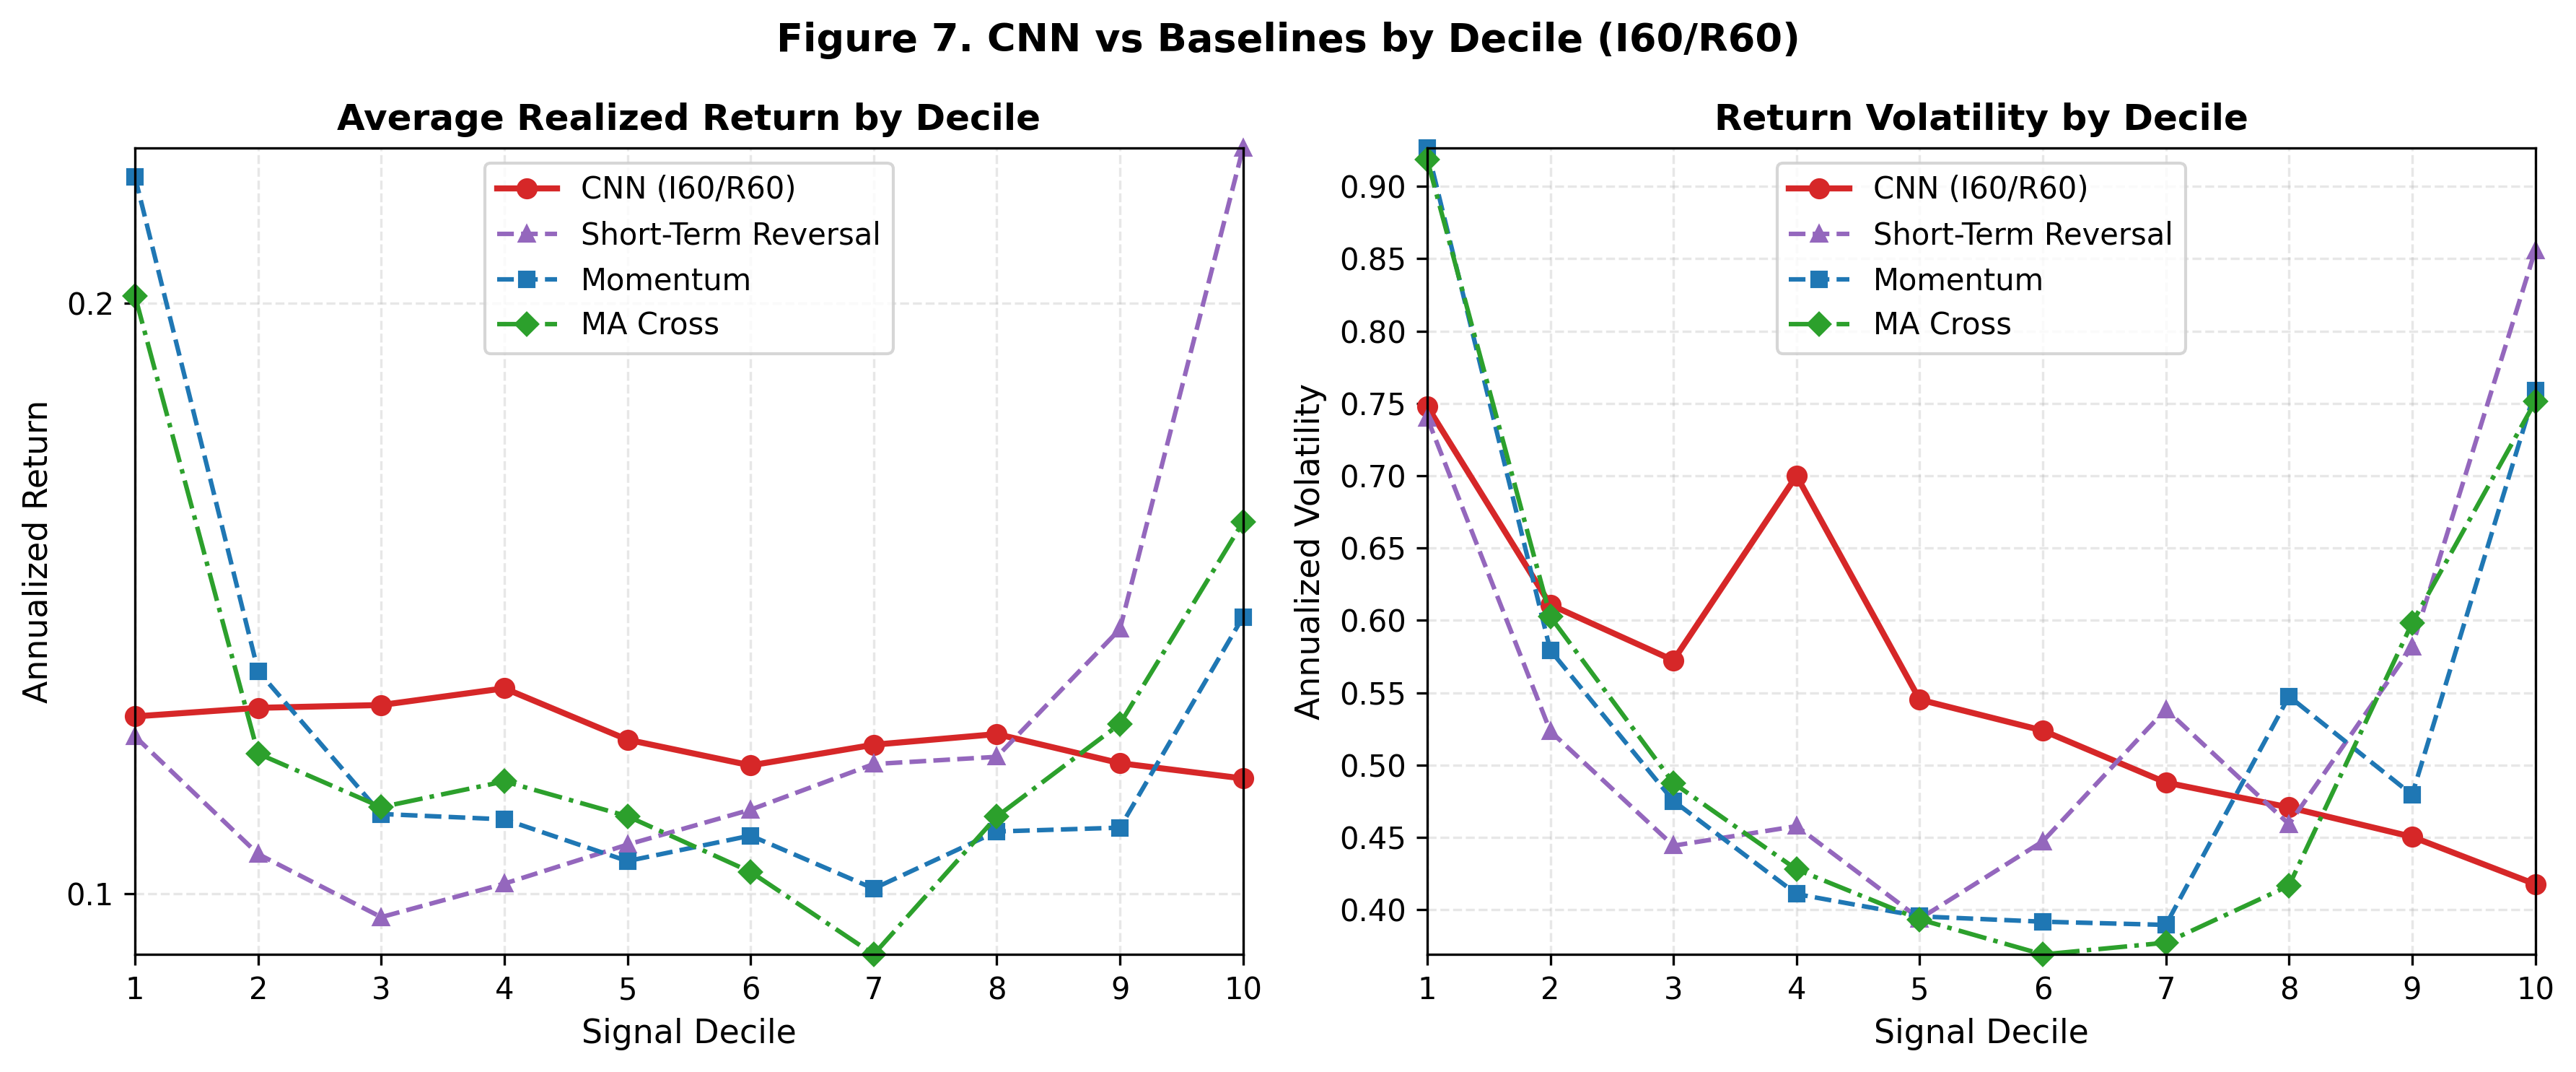
\includegraphics[width=0.82\linewidth]{fig7_I60.png}
  \caption{CNN deciles against momentum, moving-average cross, and
    short-term reversal baselines at the $I=60$ horizon. The CNN decile
    ordering is nearly flat, consistent with the attenuation of price-trend
    signals at quarterly look-back windows.}
  \label{fig:fig7-i60}
\end{figure}

\newpage
\input{checklist.tex}


\end{document}
